\chapter{SArrow: An arrow interface for writing SPar expressions} \label{chap:arrow}
When trying to express more complicated and interesting parallel patterns, e.g map or reduce, We realize SPar is too low-level so that it is difficult to express simple computation because of overheads of expressing communication patterns by hand. In addition, compilation from Par-Alg to SPar is hard since they are very different domain specific languages. 

To solve both issues, we draw inspirations from the Arrow interface (in particular, work done by \cite{braunArrowsParallelComputation2018} where they use arrow interface to express parallel computation) and introduce SArrow.

SArrow is an arrow interface for writing SPar expressions. Withe the help from SArrow, Users can use canonical arrow combinators to write algorithms in Arrow without writing any explicit communication and gain parallelized algorithms for free. Similarly, SArrow makes hassle-free compilation from Par-Alg to SPar possible because Par-Alg Proto is also an arrow expression and simply interpreting arrow combinators by the SArrow implementations fills the gap between Par-Alg and SPar. 

\section{Syntax}
\begin{listing}[ht]
\inputminted{Haskell}{arrow/def.hs} 
\caption{Definition of SArrow}
\label{SArrow:def}
\end{listing}
The simplified syntax of SArrow can be found in \coref{SArrow:def}. SArrow is a type synonym of \hask{Nat -> Pipe a b}. It consumes \hask{Nat} which means the identifier of a process and output \hask{Pipe a b}. The reson why we use \hask{Nat} as the only parameter is to ensuring no duplication of processes name since in most of the time, duplication is bad for parallelization. It will be explained more thoroughly in \secref{SArrow:roleAllc}.

\hask{Pipe a b} data structures is the essential component of SArrow. It regards computation as a pipe where data with type \hask{a} goes into the pipe and data with type \hask{b} get out of the pipe. Internally, it's a record type of four fields. \hask{start} field identifies the process where the input data is received. \hask{cont} field has the type \hask{a -> Proc} which is a continuation waiting for the input data produced by the last pipe. \hask{env} represents a group of Procs interacting inside the pipe to produce the output data, in other words, it is the parallel computation. \hask{end} indicates the process that produces the output data in the end. We can retrieve the corresponding process by a look up on the env with the key \hask{end}. The returned Proc returns a data with type \hask{b}.
\subsection{Arrow interface}
\hask{SArrow} is an instance of Arrow typeclass as well as ArrowChoice type class. For example, the type signature of the combinators \hask{>>>}, \hask{|||}, \hask{&&&} and \hask{arr} are shown below. The main difference between their type signatures and the usual arrow interface is that in the \hask{arr}, the function is wrapped with Core. In general, it captures the same meaning as the usual arrow interfaces. Implementation details of these combinators will be explained in \secref{SArrow:impl}.
\begin{code}
\begin{minted}{Haskell}
(>>>) :: SArrow a b -> SArrow b c -> SArrow a c
arr :: Core (a -> b) -> SArrow a b
(|||) :: SArrow a c -> SArrow b c -> SArrow (Either a b) c
(&&&) :: SArrow b c -> SArrow b c' -> SArrow b (c, c')
(***) :: SArrow b c -> SArrow b' c' -> SArrow (b, b') (c, c')
\end{minted}
\end{code}
\subsection{Example: Parallel programming patterns}
As an example, we will illustrate some typical computation patterns used in parallel computing.
\begin{figure}[ht]
    \centering
    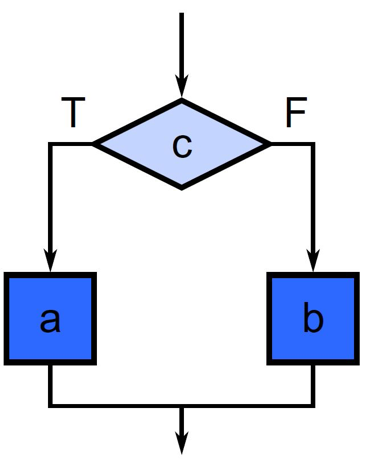
\includegraphics[width=0.3\textwidth]{arrow/select.png}
    \caption{Visualization of the branching pattern \cite{mccoolStructuredParallelPrograming2012}}
    \label{SArrow:fig:select}
\end{figure}

First of all, the branching pattern illustrated by \figref{SArrow:fig:select} is equivalent to an expression formed by \hask{|||} combinators, where the data constructor \hask{Left} leads to one computation path and the data constructor \hask{Right} leads to another computation path. It seems to be a simple pattern but it is useful when composed with other complicated patterns. We will use an example to illustrate at the end of this section.
\begin{figure*}[ht]
    \begin{subfigure}[b]{0.475\textwidth}
       \centering
       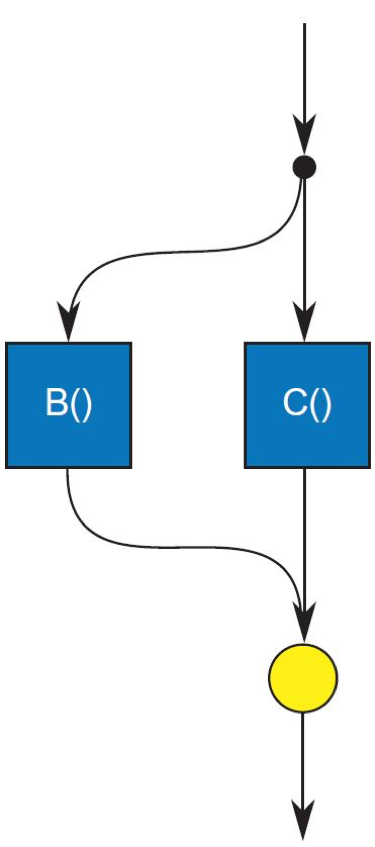
\includegraphics[width=0.60\textwidth]{arrow/fork.png}
        \caption{Visualization of the fork-join pattern \cite{mccoolStructuredParallelPrograming2012}}
        \label{SArrow:fig:fork}
    \end{subfigure}
    \hfill
   \begin{subfigure}[b]{0.475\textwidth}
        \centering
        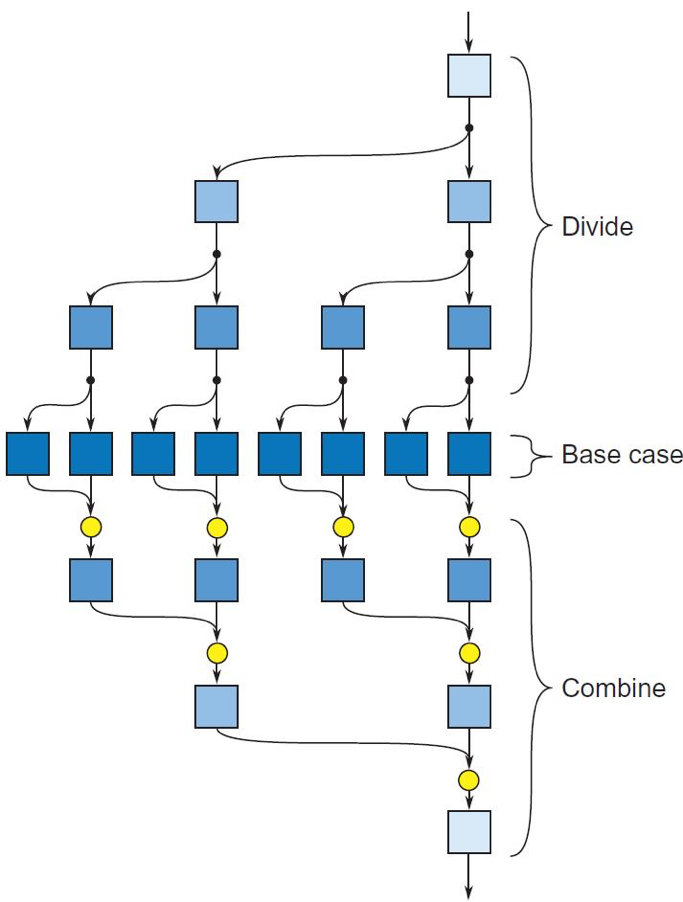
\includegraphics[width=\textwidth]{arrow/dq.png}
        \caption{Fork-Join Pattern for Divide-Conquer \cite{mccoolStructuredParallelPrograming2012}}
        \label{SArrow:fig:dq}
    \end{subfigure}
    \caption{Fork-join pattern and divide-and-conquer algorithms}
\end{figure*}
Secondly, the fundamental building block of parallel pattern, the fork-join pattern illustrated by \figref{SArrow:fig:fork} can be expressed by \hask{&&&} combinator. The SArrow produced by \hask{&&&} has the two-ary tuple as the output type collecting the computation result of the main thread and the forked thread and also acts as a synchronization point.
\begin{figure}[ht]
    \centering
    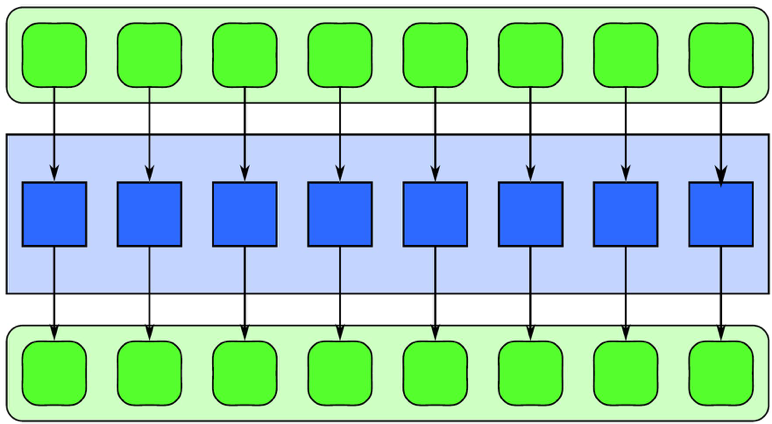
\includegraphics[width=0.5\textwidth]{arrow/pmap.png} 
    \caption{Visualization of parallel map \cite{mccoolStructuredParallelPrograming2012}}
    \label{arrow:fig:pmap}
\end{figure}
\begin{listing}[ht]
    \inputminted{Haskell}{arrow/pmap.hs}
    \caption{Parallel map in SArrow}
    \label{arrow:code:pmap}
\end{listing}
Thirdly, the familiar parallel map pattern illustrated in \figref{arrow:fig:pmap} is also a candidate to be expressed in SArrow. The code sample is in \coref{arrow:code:pmap}. \hask{pmap} splits the input \hask{a} into 4 chunks using the splitting function \hask{s}, applied the elemental function \hask{f} and the arrow combinator \hask{***} in parallel and finally use the collecting function \hask{c} to collect the results. Usually, the input \hask{a} is a list and \hask{s} splits the list into 4 equal chunks. The number of times where function is \hask{f} applied decides the number of ways of parallelism. % We will describe a possible solution to make \hask{pmap} more generic so that we do not need write a new functions for every number of ways of parallelism. (TODO).

\begin{figure}[ht]
    \centering 
    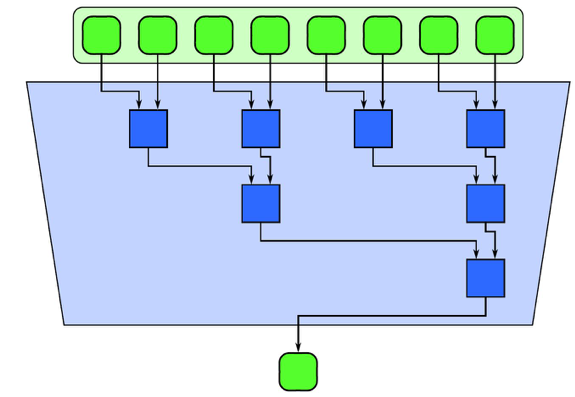
\includegraphics{arrow/preduc.png}
    \caption{Visualization of parallel reduce in SArrow \cite{mccoolStructuredParallelPrograming2012}}
    \label{arrow:fig:preduc}
\end{figure}
\begin{listing}[ht]
    \inputminted{Haskell}{arrow/preduc.hs} 
    \caption{Parallel reduce in SArrow}
    \label{arrow:code:preduc}
\end{listing}
Fourthly, we can apply the similar logic to express parallel reduce pattern shown in \figref{arrow:fig:preduc}. The code sample is in \coref{arrow:code:preduc}. The result of parallel reduce has similar type signature as the collecting function in \hask{pmap} so it is often used with the \hask{pmap} function. We use nested tuple \hask{(a, (a, (a,a)))} to represent a sized array of data. The \hask{helper} function transforms the array representation of data into a form so that we apply the reduce function \hask{r} to the elements pair-wise and parallel.

\begin{listing}[ht]
    \inputminted{Haskell}{arrow/dq.hs}
    \caption{2-ways and 3-levels divided-and-conquer algorithm in SArrow}
    \label{SArrow:dq}
\end{listing}
Finally, more complicated pattern can be expressed compositely from simpler pattern expressed in SArrow. We can use a typical divide-and-conquer algorithms implemented with fork-join as an example. \figref{SArrow:fig:dq} shows a divide-and-conquer algorithms with 2-ways and 3-levels of fork-join. The algorithm can be expressed in SArrow shown in \coref{SArrow:dq}. The divide-and-conquer pattern can be built recursively in Haskell. For the base case, we simply apply the basic computation. Otherwise, we first call split and then call the function recursively with the level decremented by one and, in the end, call the merge to combine the results. Every expressions in the function definition are connected using arrow combinators. A 3-level divided-and-conquer algorithm is constructed by passing 3 to the function resulting a algorithm with $2^3 = 8$-way parallelism.

\begin{figure}[ht]
    \centering
    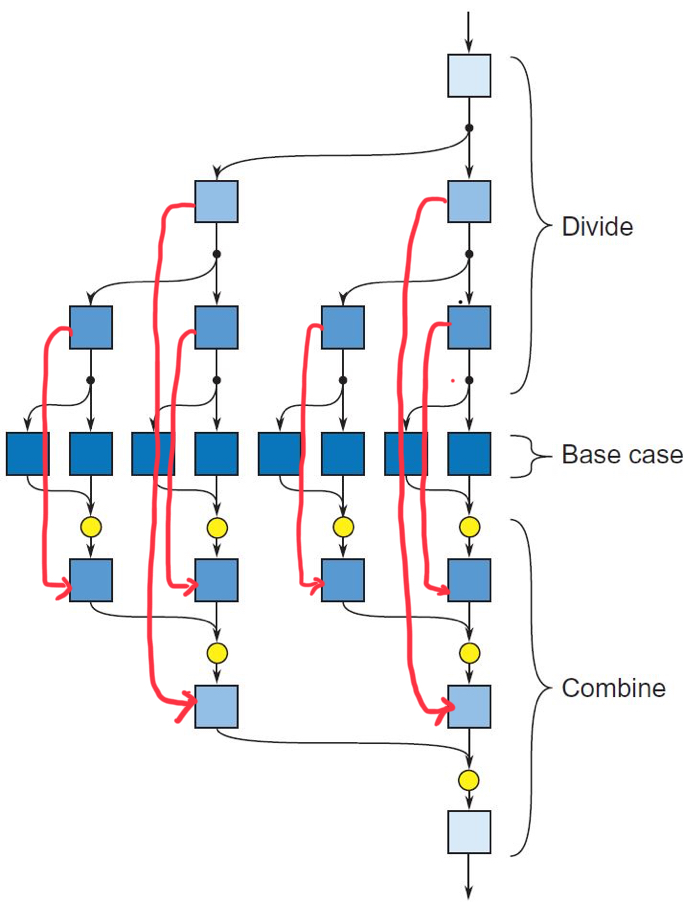
\includegraphics[width=0.5\textwidth]{arrow/dq2.jpeg}
    \caption{Combination of branching pattern and divide-and-conquer pattern}
    \label{SArrow:fig:brdv}
\end{figure}
In addition, the divide-and-conquer parallel pattern can be optimized when combining with branch pattern. The branch pattern allows us to add shortcuts to the pattern (illustrated in the \figref{SArrow:fig:brdv}, redlines represent the alternative computation path provided by branching patterns). The shortcut give us the ability to decide whether to do local computation or split  into multiple subtasks depending on the input size. When the input size is small, the overhead of the latter usually outweighs its parallelism. Adding the simple branching pattern results in a pattern that is adaptive to various input size with better performance.

The implementation demos the power of implementing SArrow as a domain specific language embedded in Haskell. We make full use of Haskell features, i.e high order functions and polymorphic functions to construct expressive, composable and generic computation patterns.

More examples of algorithms formed by SArrow, e.g. dot product or merge sort are shown in the \secref{eval}.
\section{Implementation of arrow combinators} \label{SArrow:impl}
In this chapter, we will present naive implementation and the optimized solution is introduced in the next section.

\begin{listing}[ht]
    \inputminted{Haskell}{arrow/kleisli.hs} 
    \caption{The implementation of arrow instance for Kleisli arrow of a monad}
    \label{arrow:code:kleisli}
\end{listing}
The intuition why SArrow is an instance of Arrow comes from the Kleisli arrow of a monad is an instance of Arrow class (shown in \coref{arrow:code:kleisli}). The \hask{cont} field in the Pipe has similar type signatures as the \hask{runKleisli} field in the Kleisli arrow. From the previous section, we shown that Proc is a monad so Pipe is just an extended version of Kleisli arrow where computations in Pipe usually finish in one of the process stored in \hask{env} instead of finishing at \hask{cont} like Kleisli arrow. Intuitively, SArrow, a function from the role to the Pipe, should be an instance of Arrow since Pipe looks like an arrow instance and functions are composite.

The essential issue when implementing arrow combinators is how to connect one Pipe by another Pipe. The first problem we need to address is how to deal with the \hask{cont} in the tail Pipe. We know that only one \hask{cont} field exists in the resulting Pipe and it must be that from the head Pipe. Hence the only option is to convert it to a Proc expression and store the converted expression in the updated env in the resulting Pipe. A right way to do it bind the cont with the action: receive from end in the first Pipe. Also, extend the proc related to the end in the head Porc with action: send to start in the second Pipe. Besides addition of the converted \hask{cont} expression, the new env is formed by merging the env from the head Pipe and the env from the tail Pipe. Merging two envs is trivial. When there are duplication, we simply use monadic bind to combine them so that the actions belonging to head Pipe followed by the actions belonging to the tail Pipe. The \hask{start} field in the resulting Pipe is the same as that from the head Pipe and the \hask{end} field will be set the same as that from the tail Pipe.
\begin{listing}
\inputminted{Haskell}{arrow/impl.hs}
\caption{The simplified implementation of \hask{>>>}}
\label{SArrow:code:impl}
\end{listing}
We can apply the Pipe composing function to implement arrow combinators for SArrow. The implementation is just apply the first SArrow with the input role (don't forget SArrow is a function) to get the Pipe and apply the second SArrow with a new role to get the second Pipe (usually in order to avoid duplication of roles, the new role is set to be maximum role in the first Pipe + 1) and finally apply the Pipe composing functions to both Pipe. A simplified code explanation can be seen in \coref{SArrow:code:impl}. The rest of combinators can be implemented in a similar fashion.

\section{Strategies for optimized role allocations} \label{SArrow:roleAllc}
From the last section, we know the number of roles in the system is directly related to the number of processes in the final generated code. Hence, role allocating is an essential part in generating efficient parallel programs. 

In this section, we propose strategies for optimizing role allocations. We have two goals in mind when optimizing; The first one is we would like to reduce the number of roles (processes) in the computation since the overhead of thread creation and data transmission has negative impact on performance. The second one is we do not want roles duplication when we try to compose SArrows since role duplications means the different computation must be merged in the same role and computations in the same thread is sequential hence role duplications has negative impact on degree of parallelization. 

If we only put the first goal in mind, an easy solution will be setup an upper bound of the number roles, and then we cycle through a fixed bound when allocating new roles. Processes corresponding to duplicated roles can be simply merged using binds since Proc is a monadic DSL and duality check ensures binding will not cause deadlocks. However, this strategies is not ideal since duplications of roles will decrease the degree of parallelization in the system.

If we only consider the second goal, naive strategies used in the previous section will satisfy the goal. However, the number of channels required and the number of roles in the system will grow exponentially. In a divided-and-conquer algorithm, the number of channels increases from 10 to 120 and the number of roles increases from 6 to 36 when the level is increased from 1 to 3.
\begin{listing}[ht]
\begin{displaymath} 
    \inference[id]{x: \text{Role}, \quad a: \text{Type}}{id : \text{SArrow a a}, x \Rightarrow x}
\end{displaymath}
\caption{Role allocation for id}
\label{SArrow:ra:example}
\end{listing}

For the purpose of illustration, we use inference rules to explain our proposed strategies for optimized role allocations when composing SArrows. Please see \coref{SArrow:ra:example} as an example. $x \Rightarrow x$ means the computation start with role $x$ and end with role $x$.
\begin{listing}[ht]
\begin{displaymath} 
    \inference[compose]{e1 : \text{SArrow a b}, x \Rightarrow y, \quad e2: \text{SArrow b c}, y \Rightarrow z}{e1 \; \hask{>>>} \; e2 : \text{SArrow a c}, x \Rightarrow z}
\end{displaymath}
\vskip\baselineskip
\begin{displaymath} 
    \inference[arr]{f : \text{Core (a} \rightarrow \text{b)}, \quad x: \text{Role}}{\text{arr } f: \text{SArrow a b}, x \Rightarrow x}
\end{displaymath}
\vskip\baselineskip
\begin{displaymath}
    \inference[arrow choice: \hask{|||}]{e1: \text{SArrow a c}, x \Rightarrow y, \quad e2: \text{SArrow b c}, x \Rightarrow z}{e1 \; \hask{|||}\; e2 : \text{SArrow (Either a b) c}, x \Rightarrow \text{max}(y, z)}
\end{displaymath}
\vskip\baselineskip
\begin{displaymath}
    \inference[arrow choice: \hask{+++}]{e1: \text{SArrow a c}, x \Rightarrow y, \quad e2: \text{SArrow b d}, x \Rightarrow z}{e1 \;\hask{+++}\; e2 : \text{SArrow (Either a b) (Either c d)}, x \Rightarrow \text{max}(y, z)}
\end{displaymath}
\vskip\baselineskip
\begin{displaymath}
    \inference[arrow: \hask{&&&}]{e1: \text{SArrow a b}, x \Rightarrow y, \quad e2: \text{SArrow a c}, (y+1) \Rightarrow z}{e1 \;\hask{&&&}\; e2 : \text{SArrow a (b, c)}, x \Rightarrow z}
\end{displaymath}
\vskip\baselineskip
\begin{displaymath}
    \inference[arrow: \hask{***}]{e1: \text{SArrow a b}, x \Rightarrow y, \quad e2: \text{SArrow a' c}, (y+1) \Rightarrow z}{e1 \;\hask{***}\; e2 : \text{SArrow (a, a') (b, c)}, x \Rightarrow z}
\end{displaymath}
\caption{Rules fo role allocations of different combinators}
\label{SArrow:ra:rule}
\end{listing}

The rule for the rest of combinators are shown in \coref{SArrow:ra:rule}. Notice that for compose, id, arr and ArrowChoice we do not introduce any new roles, in other words, there is no parallelization for these combinators. Reader may find it strange that we do not intent to parallelize arr combinator which lifts a sequential computation represented by Core (a $\rightarrow$ b) into SArrow. It makes sense to introduce a new role to execute the computation and hence parallelize computational heavy tasks. We use this strategy in the first place but later we found a more suitable strategy exists which will be introduced in the later paragraph. Also, another reason not to introduce new role when encountering arr combinators is that we gained function fusion for free. Simple function i.e. fst, inject left or snd are automatically fused into more complicated user defined functions. Introducing new roles for these simple functions will damage performance. % o introduce new roles when encounter \hask{&&&}. In this way, we do not sacrifice any degree of parallelization but keep the number of roles in the system at the minimum. 

For the class of combinators belonging to arrow choice, we do not introduce any new role. The expressions at the lhs and at the rhs starts with the same role $x$ because when only one code path will be executed as the name choice suggested so we should not use separate roles for two expressions that will never be executed simultaneously. In the end, we decided the computation end in the role max$(y,z)$. Max guarantees that there will not be role duplications when we compose expressions formed by ArrowChoice combinators with other combinators. For the implementation, all process in both left and right SArrow expression are wrapped inside a branch operation separately. Assume max$(y, z) = y$, the process at the role $y$ will be extended with actions that receive data from min$(y, z) = z$ role at its right branch. Finally, applying inject left and inject right at left and right branches gives us Either type as the output.

Finally, we discovered the right place to allocate new roles is \hask{&&&} combinator. As shown in type signature, product types mean computation at both branches will both be executed and they are independent. In order to make sure both computation are executed simultaneously, we constraint that the right SArrow expression must start with a role greater than the end role of the left SArrow expression. This ensures no role duplications hence maximize parallelism. The combined expression ends in the end role of the right SArrow expression instead of introducing a unnecessary new role. For the implementations, the process corresponded to end role $z$ are extended with actions that receive data from the end role $y$ of the left process and store the computation of SArrow expression at the right side and finally output a pair.

Even though from the implementation point of view, SArrow composition with the optimized role allocations is ad-hoc and less elegant to implement because we need to consider composition by send-and-receive and composition by local monadic bind and more edge cases to be dealt with compared to the naive solution in the last section where composition is done solely by send-and-receive and role allocations is mindless. We believe the effort is worthy because for a n-level divided-and-conquer algorithms, the optimized role allocation strategies allocate $2^n$ roles in total which is the same as the number of way of parallelization in theory. All the roles are used to maximize parallelism instead of wasting the valuable resources to create roles that merely transmit data.

In conclusion, the optimized strategy presented in this chapter is not the only solution. For example, there is a strategy that only introduce new roles into the computation graph when encountering a specific atomic functions. Different strategies result in different communication structures hence different kind of parallelisms. We should choose the right strategy depending on the specific task.
\section{Satisfaction of arrow laws}
We have provided the implementation of SArrow combinators that is similar to the arrow interface. However, the implementation is not enough to state that SArrow is an arrow interface. Furthermore, we need to prove that SArrow satisfy the arrow laws. Because of the limited context, we will present justification instead of formal proofs. We will focus on arrow laws. The justification for arrow-choice law can be reasoned in a similar way.
\begin{table}[ht]
    \begin{align*}
        arr(Id) >>> a &= a \tag{1}\\
        a >>> arr(Id) &= a \tag{2}\\
        (a >>> b) >>> c &= a >>> (b >>> c) \tag{3}\\
        arr(f;g) &= arr(f) >>> arr(g) \tag{4}\\
        first(a) >>> arr(Fst) &= arr(Fst) >>> a \tag{5}\\
        first(a) >>> arr(\alpha) &= arr(\alpha) >>> first(first(a)) \tag{6}\\
        first(a >>> b) =& first(a) >>> first(b) \tag{7}\\
    \end{align*}
    \caption{Arrow laws \cite{atkeyWhatCategoricalModel2011}}
    \label{arrow:tab:law}
\end{table}

\tabref{arrow:tab:law} shows the rules of arrow laws. We includes a subset of law that contains the \hask{first} combinator. The other half of laws that contains the \hask{second} combinator can be proved by symmetry. \hask{first} combinator is implemented as \hask{first = (*** id)} and $\alpha :: ((x, y), z) -> (x, (y, z))$.
\begin{figure}[ht]
    \centering
    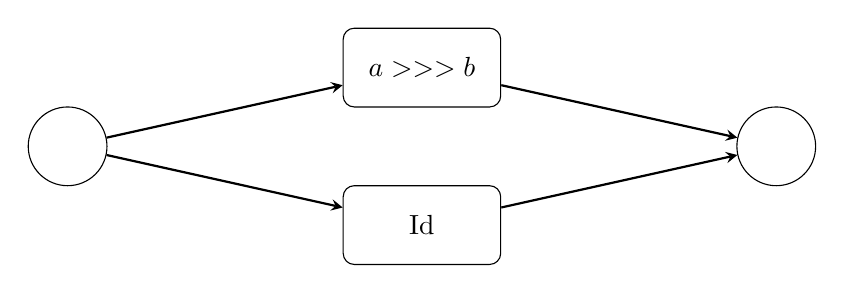
\begin{tikzpicture}[xscale=1.5]
        \tikzstyle{proc} = [rectangle, rounded corners, minimum width=2cm, minimum height=1cm,text centered, draw=black] 
        \tikzstyle{proc1} = [circle,  minimum width=1cm, minimum height=1cm,text centered, draw=black] 
        \tikzstyle{arrow} = [thick,->,>=stealth]
        \node (a) [proc1] at (0, 0) {};
        \node (c) [proc] at (3, 1) {$a >>> b$};
        \node (d) [proc1] at (6, 0) {};
        \node (e) [proc] at (3, -1) {Id};
        \draw[arrow] (a) to (c);
        \draw[arrow] (c) to (d);
        \draw[arrow] (a) to (e);
        \draw[arrow] (e) to (d);
    \end{tikzpicture}
    \vskip\baselineskip
    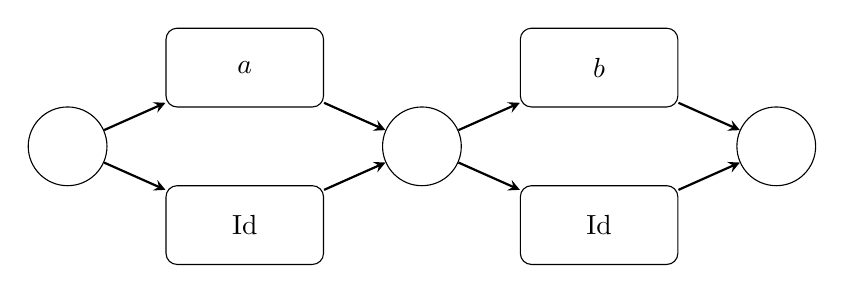
\begin{tikzpicture}[xscale=1.5]
        \tikzstyle{proc} = [rectangle, rounded corners, minimum width=2cm, minimum height=1cm,text centered, draw=black] 
        \tikzstyle{proc1} = [circle,  minimum width=1cm, minimum height=1cm,text centered, draw=black] 
        \tikzstyle{arrow} = [thick,->,>=stealth]
        \node (a) [proc1] at (0, 0) {};
        \node (c) [proc] at (1.5, 1) {$a$};
        \node (d) [proc1] at (3, 0) {};
        \node (e) [proc] at (1.5, -1) {Id};
        \node (f) [proc] at (4.5, 1) {$b$};
        \node (g) [proc] at (4.5, -1) {Id};
        \node (h) [proc1] at (6, 0) {};
        \draw[arrow] (a) to (c);
        \draw[arrow] (c) to (d);
        \draw[arrow] (a) to (e);
        \draw[arrow] (e) to (d);
        \draw[arrow] (d) to (f);
        \draw[arrow] (d) to (g);
        \draw[arrow] (f) to (h);
        \draw[arrow] (g) to (h);
    \end{tikzpicture}
    \caption{Graphical representation of equation (7)}
    \label{arrow:fig:eq7}
\end{figure}

\begin{figure}[ht]
    \centering
    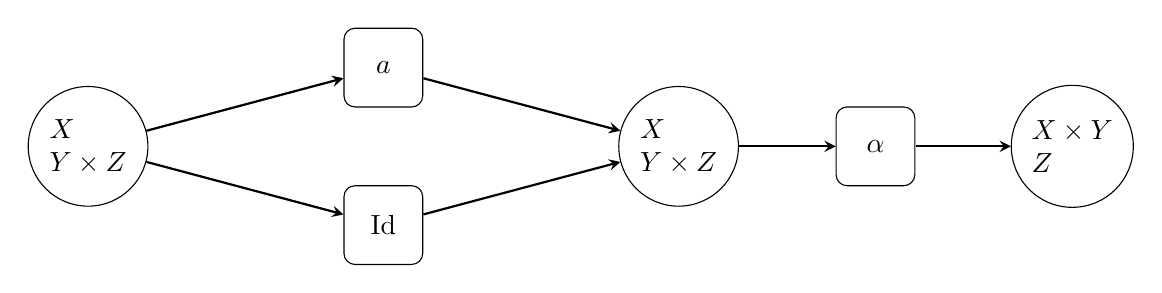
\begin{tikzpicture}[xscale=2.5]
        \tikzstyle{proc} = [rectangle, rounded corners, minimum width=1cm, minimum height=1cm,text centered, draw=black] 
        \tikzstyle{proc1} = [circle,  minimum width=1cm, minimum height=1cm,text centered, draw=black] 
        \tikzstyle{arrow} = [thick,->,>=stealth]
        \node [proc1, align=left] (2) at (0, 0) {$X$ \\ $Y \times Z$};
	 \node [proc] (3) at (1.5, 1) {$a$};
	 \node [proc] (4) at (1.5, -1) {Id};
	 \node [proc] (7) at (4, 0) {$\alpha$};
	 \node [proc1, align=left] (8) at (5, 0) {$X \times Y$ \\ $Z$};
	 \node [proc1, align=left] (9) at (3, 0) {$X$ \\ $Y \times Z$};
     \draw[arrow] (2) to (3);
     \draw[arrow] (3) to (9);
     \draw[arrow] (2) to (4);
     \draw[arrow] (4) to (9);
     \draw[arrow] (9) to (7);
     \draw[arrow] (7) to (8);
    \end{tikzpicture}
    \vskip\baselineskip
    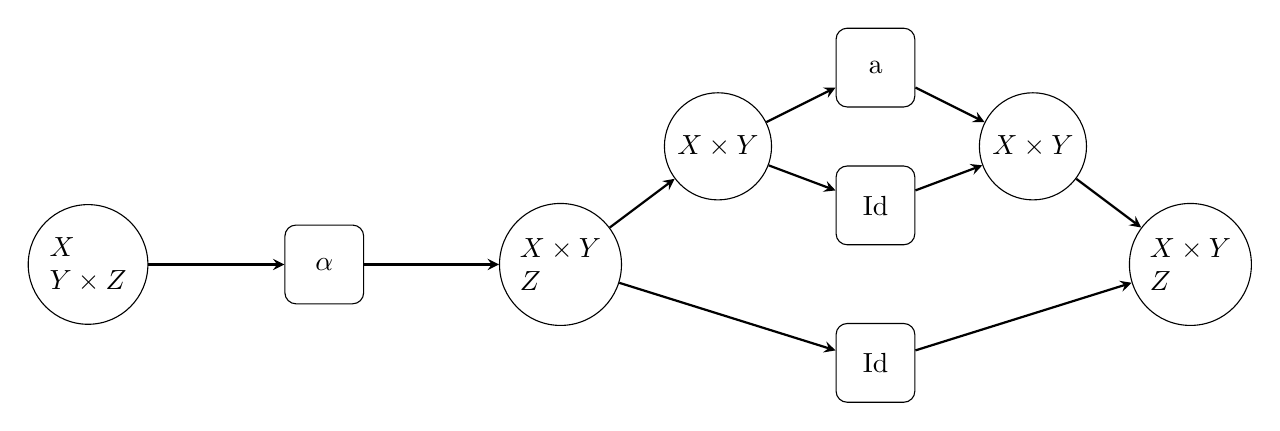
\begin{tikzpicture}[xscale=2.0]
        \tikzstyle{proc} = [rectangle, rounded corners, minimum width=1cm, minimum height=1cm,text centered, draw=black] 
        \tikzstyle{proc1} = [circle,  minimum width=1cm, minimum height=1cm,text centered, draw=black] 
        \tikzstyle{arrow} = [thick,->,>=stealth]
		\node [proc1, align=left] (0) at (-1, 0) {$X$ \\ $Y \times Z$};
		\node [proc] (1) at (0.5, 0) {$\alpha$};
		\node [proc1, align=left] (2) at (2, 0) {$X \times Y$ \\ $Z$};
		\node [proc] (5) at (4, 2.5) {a};
		\node [proc] (6) at (4, 0.75) {Id};
		\node [proc1] (7) at (5, 1.5) {$X \times Y$};
		\node [proc1, align=left] (8) at (6, 0) {$X \times Y$ \\ $Z$};
		\node [proc1] (9) at (3, 1.5) {$X \times Y$};
		\node [proc] (10) at (4, -1.25) {Id};
		\draw[arrow] (0) to (1);
		\draw[arrow] (1) to (2);
		\draw[arrow] (2) to (9);
		\draw[arrow] (9) to (5);
		\draw[arrow] (9) to (6);
		\draw[arrow] (5) to (7);
		\draw[arrow] (6) to (7);
		\draw[arrow] (7) to (8);
		\draw[arrow] (2) to (10);
        \draw[arrow] (10) to (8);
    \end{tikzpicture}
    \caption{Graphical representation of equation (6)}
    \label{arrow:fig:eq6}
\end{figure}

We argue above equation holds if both sides of equation express the same computation. Equation (1), (2) holds because lifting Id from Core to SArrow will not modify the result of computation due to the semantics of Id. Equation (3) is the associativity rule of $>>>$. Left side of the equation sends the output from $a >>> b$ to the input of $c$ while right side sends the output of $a$ to the input $b >>> c$. The communication structure might change but they both represents the same computation. Equation (4) is valid because applying the input value to composition of f;g is the same as applying the input to f followed by a message passing (data communication could be local which means the communication structure for both side of equations are the same in this case) and then applying it to g. One might claim that the left side is more efficient than the right side due to the fusion depending on the role allocation strategy. Equation (5) holds because they both represents a computation that take a pair input and apply the function a to its first position and return the result. Right hand side of equation (7) represents a SArrow expression that applies a on left position of input pair and applies Id on the right position of input pair in parallel, collects the results and applies b on left position of input pair and applies Id on the right position of input pair while left side fused a and b together and apply them in one step hence there is only one join point. \figref{arrow:fig:eq7} is a graphical representation of equation (7). Obviously they represents the same computation. We can also derive equation (6) from its Visualization (see in \figref{arrow:fig:eq6}).

\section{Conclusions}
Arrow interface is the perfect interface to express general computation for this project because not only is it intuitive to understand and visualize but also its combinators \hask{***} and \hask{&&&} has built-in parallel natural.

So far, we've used SArrow to help us compile Par-Alg to SPar. The remained challenge is the code generation from SPar to a target platform. In the next chapter, we will introduce our methods for code generation and specifically code generation to C. Once we achieved this, every computation in SArrow can be transformed into parallel C code in one step.

% \section{Applications}
% \subsection{Hassle-free compilation from ParAlg to SArrow} %Hassle-free
% \subsection{An interface for arrow computation with automatic parallelization}
% \section{Power of arrow and EDSL: &)expressibility and composability}
% \subsection{Arrow interface}
% \subsection{Haskell as the host language}